\documentclass[12pt, a4paper]{article} %determina o tamanho da fonte, o tipo de papel e o tipo de documento.

\setlength{\parindent}{1.0 cm} %tamanho do espa\c{c}o para come\c{c}ar o parágrafo.
\setlength{\parskip}{0.5cm} %tamanho do espa\c{c}o entre os parágrafos.

%Aqui ficam os pacotes utilizados para formata\c{c}\~ao do documento de modo geral:

\usepackage[utf8]{inputenc} 
\usepackage{indentfirst} %Coloca espa\c{c}os nos inícios de parágrafos automaticamente. 
\usepackage[brazilian]{babel} %
\usepackage{amsmath}
\usepackage[hmargin=3cm, vmargin=2.5cm, bmargin=2.5cm]{geometry}
\usepackage{multicol}
\usepackage{graphicx} %para poder inserir imagens
\usepackage{subfig}
\usepackage{booktabs} 
\usepackage{hyperref} %para poder adicionar links e hiperlinks
\usepackage{float} %para poder posicionar as imagens
\usepackage{subfig} %para colocar duas imagens juntas

\usepackage{listings} %para poder incluir códigos
\usepackage{xcolor}
\definecolor{codegreen}{rgb}{0,0.6,0}
\definecolor{codegray}{rgb}{0.5,0.5,0.5}
\definecolor{codepurple}{rgb}{0.58,0,0.82}
\definecolor{backcolour}{rgb}{0.95,0.95,0.92}
\lstdefinestyle{mystyle}{
    backgroundcolor=\color{backcolour},   
    commentstyle=\color{codegreen},
    keywordstyle=\color{magenta},
    numberstyle=\tiny\color{codegray},
    stringstyle=\color{codepurple},
    basicstyle=\ttfamily\footnotesize,
    breakatwhitespace=false,         
    breaklines=true,                 
    captionpos=b,                    
    keepspaces=true,                 
    numbers=left,                    
    numbersep=5pt,                  
    showspaces=false,                
    showstringspaces=false,
    showtabs=false,                  
    tabsize=2,
    morecomment={l}[!],
    language=[77]Fortran,
}
\lstset{style=mystyle}

\begin{document} %come\c{c}a alguma coisa,neste caso, o documento, sempre importante lembrar de colocar o \end{} para n\~ao dar erro 
	
	\begin{titlepage}
		\begin{center}
\Huge{Universidade de S\~ao Paulo}\\
\large{Instituto de Física de S\~ao Carlos}\\
\vspace{20pt}
\vspace{200pt}
\textbf{Projeto 2}\\
\vspace{8cm}
		\end{center}

\begin{flushleft}
\begin{tabbing}
Pedro Calligaris Delbem 5255417\\
\end{tabbing}
\vspace{0.5cm}
Professor: Attilio Cucchieri\\		
		\end{flushleft}
	
		\begin{center}
			\vspace{\fill}
	Junho de 2025	
		\end{center}
	\end{titlepage}

%####################################################################### SUMÁRIO
	\tableofcontents 
	\thispagestyle{empty}
	\newpage
%#########################################################################

    \section{Exerc\'icio 1}

        Tarefa: Na lista 5, foi considerado o po\c{c}o de potencial infinito no intervalo $[0, L]$, para uma part\'icula de massa $m$, ou seja, a equac\c{c}\~ao
        \begin{equation}
            -\frac{\hbar^{2}}{2m}\nabla^{2}\psi_{j}(x)=E_{j}\psi_{j}(x).
        \end{equation}
        Para encontrar as autofun\c{c}\~oes
        \begin{equation*}
            \psi_{j}(x) \propto \sin\left(\frac{j\pi x}{L}\right)
        \end{equation*}
         foi considerada a matriz
        \[
        \begin{pmatrix}
            -2 & 1 & 0 & \cdots & 0 \\
            1 & -2 & 1 & \cdots & 0 \\
            0 & 1 & -2 & \cdots & 0 \\
            \vdots & \vdots & \ddots & \ddots & \vdots \\
            0 & 0 & 0 & 1 & -2
        \end{pmatrix}
        \]
        Agora, considere a matriz
        \begin{equation}
        \begin{pmatrix}
            -1 & 1 & 0 & \cdots & 0 \\
            1 & -2 & 1 & \cdots & 0 \\
            0 & 1 & -2 & \cdots & 0 \\
            \vdots & \vdots & \ddots & \ddots & \vdots \\
            0 & 0 & 0 & 1 & -2
        \end{pmatrix}
        \end{equation}
        Que tipo de soluc\c{c}\~oes para o po\c{c}o de potencial infinito voc\^e espera encontrar nesse caso? Motive sua resposta.
        
        \textbf{Resposta:}

        Para um ponto no extremo inicial da grade, a discretiza\c{c}\~ao de diferen\c{c}as finitas para a primeira derivada \'e:
        \begin{equation}
            \frac{d\psi}{dx} \bigg|_{x=0} \approx \frac{\psi_1 - \psi_0}{h}
        \end{equation}
        A Condi\c{c}\~ao de Contorno de Neumann é:
        \begin{equation}
            \frac{d\psi}{dx} \bigg|_{x=0} = 0
        \end{equation}
        O que nos leva a
        \begin{equation}
            \psi_0 = \psi_1
        \end{equation}
        Substituindo isto na discretiza\c{c}\~ao de diferen\c{c}as finitas para a segunda derivada - no ponto $x_i$, temos:
        \begin{equation}
            \frac{d^2\psi}{dx^2} \bigg|_{x=x_1} \approx \frac{\psi_2 - 2\psi_1 + (\psi_1)}{h^2} = \frac{\psi_2 - \psi_1}{h^2}
        \end{equation}
        Que resulta em dois termos, justamente com os coeficientes -1 e 1, que temos na matriz dada.
        Logo, espera-se que a solu\c{c}\~ao seja tal que obede\c{c}a a condi\c{c}\~ao de contorno de Neumann e portanto o resultado ser\'a:
        \begin{equation*}
            \psi_{j}(x) \propto \cos\left(\frac{j\pi x}{2L}\right)
        \end{equation*}

    \section{Exercício 2}

        Tarefa: Usando o \textit{power method} e a matriz (2), calcule a energia do estado fundamental $E_{0}$ com precis\~ao de $10^{-4}$. Compare o resultado com o valor exato. Fa\c{c}a um gr\'afico da autofunc\c{c}\~ao normalizada e compare com a soluc\c{c}\~ao exata.

        O c\'odigo foi compilado com o comando:

    gfortran -ffree-form -ffree-line-length-none P2-5255417-ex-2.f90 -Wall -Wextra -pedantic -o P2-5255417-ex-2.exe

        Resultados:

        Utilizou-se N=100000 como se fosse N=infinito, obtendo a energia:
        \begin{figure}[H]
            \centering
            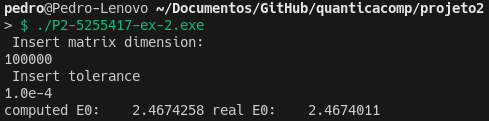
\includegraphics[width=0.8\textwidth]{../images/ex2.png}
        \end{figure}
        E obteve-se a seguinte autofun\c{c}\~ao:
        \begin{figure}[H]
            \centering
            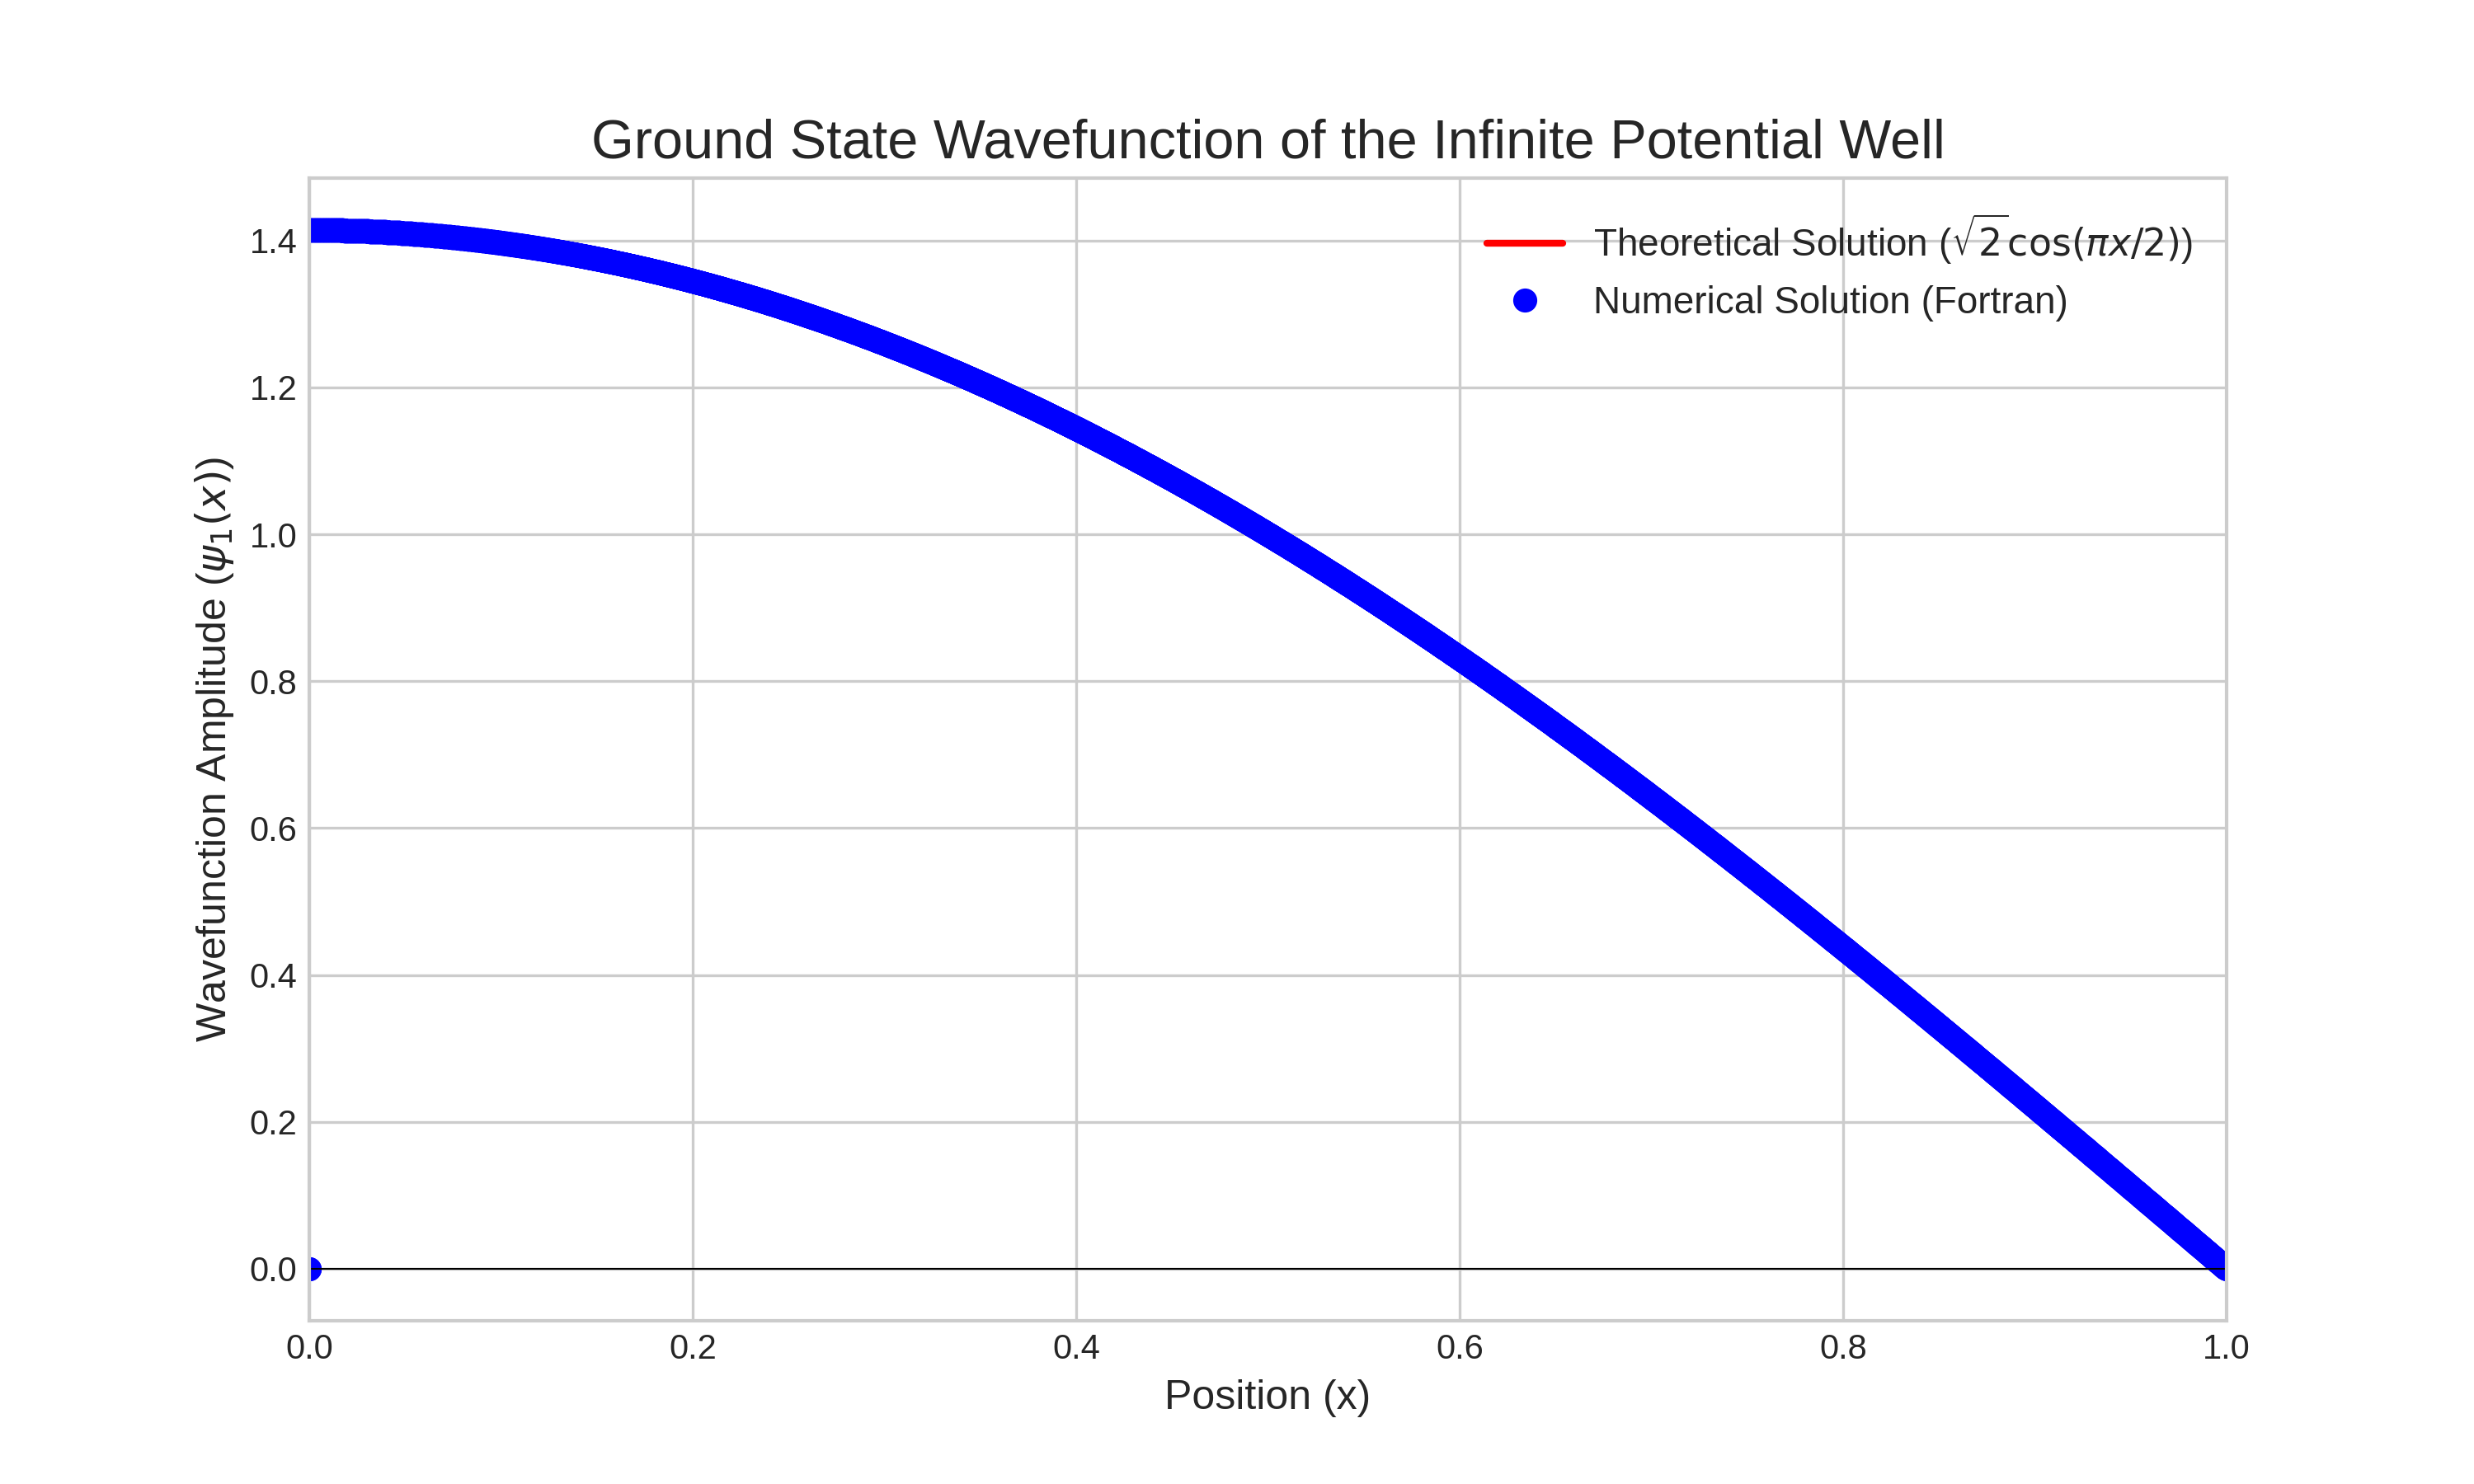
\includegraphics[width=0.8\textwidth]{../images/wavefunction_plot.png}
        \end{figure}

        V\^e-se que a fun\c{c}\~ao anal\'itica e a num\'erica se sobrep\~oe totalmente, de modo que o m\'etodo num\'erico corresponde perfeitamente à fun\c{c}\~ao anal\'itica conhecida. (O autovetor resultante foi salvo no arquivo "P2-5255417-ex-2-results.txt")

    \section{Exerc\'icio 3}

        Tarefa: Considere o m\'etodo de Householder, estudado na lista 6. Naquele caso, para os elementos fora da diagonal $k_{i}$, foi usado o sinal oposto de $a_{i-1,i}$. O que acontece quando o sinal de $k_{i}$ \'e o mesmo de $a_{i-1,i}$? Estude o problema para a mesma matriz considerada na lista 6, ou seja
        \[
        A =
        \begin{pmatrix}
        -\frac{5}{2} & \frac{4}{3} & -\frac{1}{12} & 0 & 0 & 0 \\
        \frac{4}{3} & -\frac{5}{2} & \frac{4}{3} & -\frac{1}{12} & 0 & 0 \\
        -\frac{1}{12} & \frac{4}{3} & -\frac{5}{2} & \frac{4}{3} & -\frac{1}{12} & 0 \\
        0 & -\frac{1}{12} & \frac{4}{3} & -\frac{5}{2} & \frac{4}{3} & -\frac{1}{12} \\
        0 & 0 & -\frac{1}{12} & \frac{4}{3} & -\frac{5}{2} & \frac{4}{3} \\
        0 & 0 & 0 & -\frac{1}{12} & \frac{4}{3} & -\frac{5}{2}
        \end{pmatrix}
        \]
        Qual \'e a relac\c{c}\~ao entre a matriz tridiagonal obtida neste caso e a matriz tridiagonal obtida na lista 6?
        
        Os c\'odigos foram compilados com os comandos (original e modificado --- respectivamente):

        \begin{itemize}
            \item gfortran -ffree-form -ffree-line-length-none P2-5255417-ex-3a.f90 -Wall -Wextra -pedantic -o P2-5255417-ex-3a.exe

            \item gfortran -ffree-form -ffree-line-length-none P2-5255417-ex-3b.f90 -Wall -Wextra -pedantic -o P2-5255417-ex-3b.exe
        \end{itemize}
                
        Resultados:

        \begin{figure}[H]
            \centering
            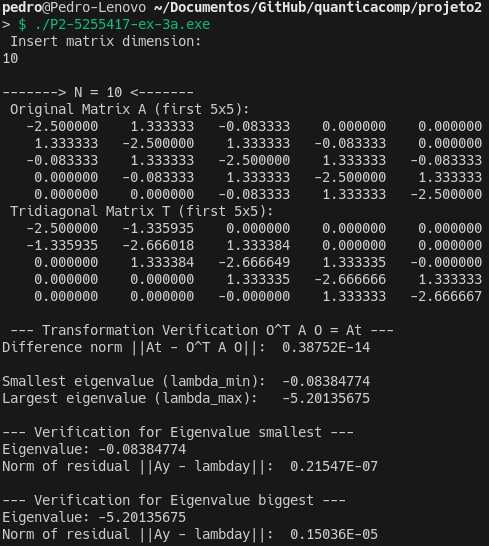
\includegraphics[width=0.8\textwidth]{../images/ex3a-10.png}
        \end{figure}
        \begin{figure}[H]
            \centering
            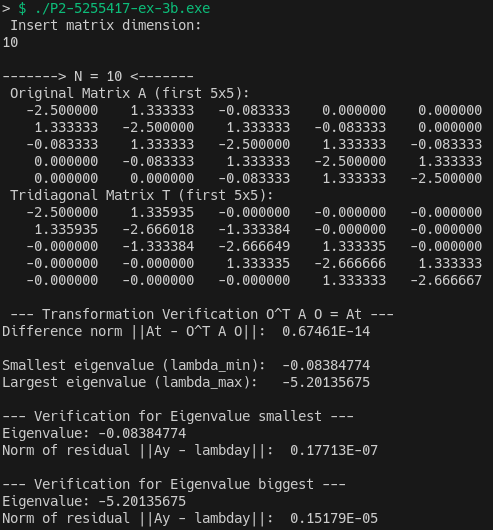
\includegraphics[width=0.8\textwidth]{../images/ex3b-10.png}
        \end{figure}
        \begin{figure}[H]
            \centering
            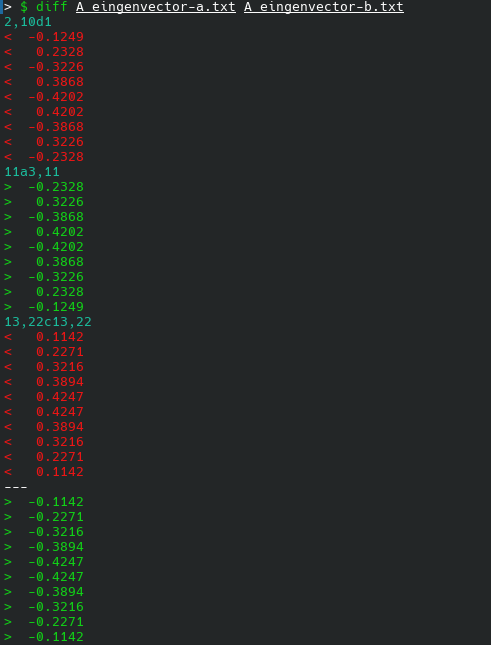
\includegraphics[width=0.8\textwidth]{../images/diffA10.png}
        \end{figure}
        \begin{figure}[H]
            \centering
            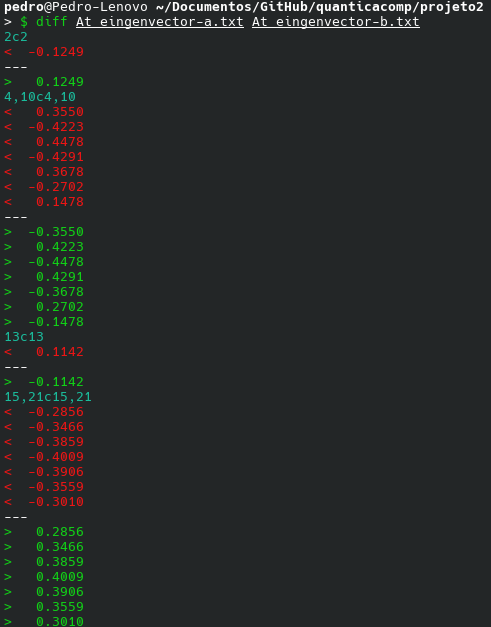
\includegraphics[width=0.8\textwidth]{../images/diffAt10.png}
        \end{figure}

        Nota-se que todas as verifica\c{c}\~oes - em ambos os c\'odigos - resultaram em valores pequenos, mostrando que o m\'etodo funcionou bem para ambos os c\'odigos.
            
        Entretando, ao comparar os arquivos que cont\^em os autovetores resultantes ("At\_eingenvector-a.txt" e "A\_eingenvector-a.txt" para o sinal original e "At\_eingenvector-b.txt" e "A\_eingenvector-b.txt" para o sinal modificado) - al\'em de comparar as matrizes impressas como resultado dos c\'odigos -  percebe-se que há uma diferen\c{c}a de sinal em alguns elementos da matriz (al\'em de uma pequena diferen\c{c}a no valor absoluto de alguns elementos), enquanto os autovetores apresentam - al\'em da diferen\c{c}a de sinal - uma invers\~ao da "ordem" dos elementos (apesar de serem os mesmos).
        
        Deste modo, percebe-se que o m\'etodo funcionou bem para ambos os sinais - encontrando, para cada sinal, uma das duas solu\c{c}\~oes poss\'iveis. O erro esperado - devido ao erro de subtra\c{c}\~ao num\'erica - n\~ao foi um problema devido a um "bom comportamento" da matriz.

    \section{Exerc\'icio 4}

        Tarefa: Considere novamente o problema da lista 6. Tente resolv\^e-lo usando a menor quantidade poss\'ivel de mem \'oria. Indique, em fun\c{c}\~ao do tamanho n da matriz, qual \'e a quantidade de espa\c{c}o de mem\'oria utilizado pelas vari\'aveis (do tipo real) no programa 3

        O c\'odigo foi compilado com o comando:

    gfortran -ffree-form -ffree-line-length-none P2-5255417-ex-4.f90 -Wall -Wextra -pedantic -o P2-5255417-ex-4.exe

        \subsection*{Modifica\c{c}\~oes Feitas no Algoritmo}

        As seguintes altera\c{c}\~oes foram implementadas para passar de uma abordagem com alto consumo de mem\'oria para uma otimizada:

        \begin{enumerate}
            \item \textbf{Elimina\c{c}\~ao da Matriz de Transforma\c{c}\~ao (\texttt{O}):} A mudan\c{c}a mais significativa foi deixar de construir e armazenar a matriz de transforma\c{c}\~ao ortogonal expl\'icita $O$ (de tamanho $n \times n$).

            \item \textbf{Elimina\c{c}\~ao da C\'opia da Matriz Original (\texttt{A}):} A c\'opia da matriz original, que era mantida para verifica\c{c}\~oes, foi removida. O algoritmo agora opera ``in-place'' em uma \'unica matriz (\texttt{At}).

            \item \textbf{Armazenamento Impl\'icito dos Vetores de Householder:} Em vez de descartar os vetores de Householder $u_k$ a cada passo, suas informa\c{c}\~oes essenciais s\~ao agora armazenadas:
            \begin{itemize}
                \item Uma parte do vetor $u_k$ (os elementos de $u_{k+2}$ em diante) \'e guardada na parte triangular inferior da matriz \texttt{At}, aproveitando o espa\c{c}o que \'e zerado pelo pr\'oprio algoritmo.
                \item O primeiro elemento de cada vetor $u_k$ (\texttt{u1\_storage}) e o escalar de transforma\c{c}\~ao $\beta_k$ (\texttt{betas}) s\~ao guardados em dois novos vetores auxiliares de dimens\~ao $n$.
            \end{itemize}

            \item \textbf{Cria\c{c}\~ao da Sub-rotina \texttt{backward\_transformation}:} Uma nova sub-rotina foi criada com a finalidade de aplicar as transforma\c{c}\~oes de Householder em ordem inversa ($P_{n-2}, \dots, P_1$) diretamente no autovetor \texttt{yt}. Ela reconstr\'oi cada transforma\c{c}\~ao a partir das informa\c{c}\~oes salvas e substitui a opera\c{c}\~ao \texttt{matmul(O, yt)}.
            
            \item \textbf{Elimina\c{c}\~ao de Matrizes e Vetores Tempor\'arios:} Para a otimiza\c{c}\~ao m\'axima de mem\'oria, a fun\c{c}\~ao \texttt{outer\_product} foi removida. A atualiza\c{c}\~ao da matriz na sub-rotina de Householder foi reescrita com um la\c{c}o expl\'icito, evitando a aloca\c{c}\~ao de matrizes tempor\'arias de tamanho $n \times n$. Adicionalmente, o vetor de trabalho \texttt{q} foi eliminado, reutilizando-se o vetor \texttt{p} para os c\'alculos.
            
            \item \textbf{Adapta\c{c}\~ao da Verifica\c{c}\~ao:} Para cumprir o requisito de verificar a transforma\c{c}\~ao, a sub-rotina (\texttt{verify\_transformation}) foi modificada. Em vez de reconstruir a matriz \texttt{O} e usar $O(n^2)$ de mem\'oria, esta rotina verifica a identidade matem\'atica equivalente $A \cdot O = O \cdot A_t$ coluna por coluna, utilizando apenas vetores tempor\'arios de tamanho $O(n)$.

        \end{enumerate}

        \subsection*{Compara\c{c}\~ao do Uso de Mem\'oria}

            \subsection*{Vers\~ao Antiga (N\~ao Otimizada)}

            Nesta vers\~ao, o programa mant\'em m\'ultiplas c\'opias da matriz e constr\'oi explicitamente a matriz de transforma\c{c}\~ao $O$.

            \subsubsection*{1. Vari\'aveis Alocadas no Programa Principal (Globais)}
            Estas vari\'aveis existem durante toda a execu\c{c}\~ao do programa.
            \begin{itemize}
                \item Matriz Original \texttt{A}: $n^2$ elementos
                \item Matriz de Trabalho \texttt{At}: $n^2$ elementos
                \item Matriz de Transforma\c{c}\~ao \texttt{O}: $n^2$ elementos
                \item Vetores de Diagonais \texttt{d}, \texttt{e}: $2n$ elementos
                \item Vetores de Autovetores \texttt{yt\_min/max}, \texttt{y\_min/max}: $4n$ elementos
            \end{itemize}
            \textbf{Subtotal (Globais):} $3n^2 + 6n$ elementos.

            \subsubsection*{2. Pico de Mem\'oria Local (Dentro de Sub-rotinas)}
            A mem\'oria de pico ocorre quando o programa principal chama a sub-rotina que mais aloca mem\'oria localmente, neste caso, a \texttt{verify\_transformation}.
            \begin{itemize}
                \item Matriz \texttt{C}: $n^2$ elementos
                \item Matriz \texttt{TEMP}: $n^2$ elementos
            \end{itemize}
            \textbf{Pico Local:} $2n^2$ elementos.

            \subsubsection*{Total de Mem\'oria de Pico (Vers\~ao Antiga)}
            A mem\'oria total de pico \'e a soma das vari\'aveis globais mais o pico de aloca\c{c}\~ao local.
            \[
            M_{\text{antiga}}(n) = \underbrace{(3n^2 + 6n)}_{\text{Globais}} + \underbrace{2n^2}_{\text{Pico Local}} = 5n^2 + 6n
            \]
            Em bytes (assumindo 8 bytes por \texttt{real(dp)}):
            \[
            \text{Mem\'oria}_{\text{antiga}} = (5n^2 + 6n) \times 8 \text{ bytes}
            \]

            \subsection*{Vers\~ao Nova (Otimizada)}

            Nesta vers\~ao, as matrizes \texttt{A} e \texttt{O} s\~ao eliminadas. A informa\c{c}\~ao da transforma\c{c}\~ao \'e guardada em vetores.

            \subsubsection*{1. Vari\'aveis Alocadas no Programa Principal (Globais)}
            \begin{itemize}
                \item Matriz de Trabalho \texttt{At}: $n^2$ elementos
                \item Vetores de Diagonais \texttt{d}, \texttt{e}: $2n$ elementos
                \item Vetores de Autovetores \texttt{yt\_min/max}, \texttt{y\_min/max}: $4n$ elementos
                \item Vetores Auxiliares \texttt{betas}, \texttt{u1\_storage}: $2n$ elementos
            \end{itemize}
            \textbf{Subtotal (Globais):} $n^2 + 8n$ elementos.

            \subsubsection*{2. Pico de Mem\'oria Local (Dentro de Sub-rotinas)}
            O pico de aloca\c{c}\~ao local agora ocorre na nova sub-rotina de verifica\c{c}\~ao, \texttt{verify\_transformation\_min\_memory}.
            \begin{itemize}
                \item Vetor \texttt{previous\_O\_column}: $n$ elementos
                \item Vetor \texttt{current\_O\_column}: $n$ elementos
                \item Vetor \texttt{next\_O\_column}: $n$ elementos
                \item Vetor \texttt{left\_hand\_side\_column}: $n$ elementos
                \item Vetor \texttt{right\_hand\_side\_column}: $n$ elementos
                \item Vetor \texttt{basis\_vector}: $n$ elementos
            \end{itemize}
            \textbf{Pico Local:} $6n$ elementos.

            \subsubsection*{Total de Mem\'oria de Pico (Vers\~ao Otimizada)}
            A mem\'oria total de pico \'e a soma das novas vari\'aveis globais mais o novo pico de aloca\c{c}\~ao local.
            \[
            M_{\text{otimizada}}(n) = \underbrace{(n^2 + 8n)}_{\text{Globais}} + \underbrace{6n}_{\text{Pico Local}} = n^2 + 14n
            \]
            Em bytes:
            \[
            \text{Mem\'oria}_{\text{otimizada}} = (n^2 + 14n) \times 8 \text{ bytes}
            \]

            \subsubsection*{An\'alise Focada na Sub-rotina \texttt{householder\_reduction}}

                Para isolar o impacto direto da otimiza\c{c}\~ao, podemos comparar a mem\'oria total (argumentos + vari\'aveis locais) utilizada apenas pela sub-rotina de Householder em cada vers\~ao.

                \begin{table}[H]
                \centering
                \caption{Compara\c{c}\~ao de Mem\'oria - Apenas Sub-rotina Householder}
                \begin{tabular}{|l|c|}
                \hline
                \textbf{Vers\~ao da Sub-rotina} & \textbf{F\'ormula de Mem\'oria (elementos)} \\
                \hline
                Antiga (n\~ao otimizada) & $2n^2 + 4n$ \\
                Otimizada & $n^2 + 4n$ \\
                \hline
                \end{tabular}
                \end{table}

                Esta tabela mostra que a otimiza\c{c}\~ao reduziu o consumo de mem\'oria quadr\'atico da pr\'opria sub-rotina em 50\%, ao eliminar a necessidade de passar a matriz de transforma\c{c}\~ao \texttt{O} como argumento.

            \subsection*{Conclus\~ao Comparativa}

            \begin{table}[h!]
            \centering
            \begin{tabular}{|l|c|c|}
            \hline
            \textbf{Vers\~ao} & \textbf{F\'ormula de Mem\'oria (elementos)} & \textbf{Termo Dominante} \\
            \hline
            Antiga & $5n^2 + 6n$ & $5n^2$ \\
            Otimizada & $n^2 + 14n$ & $n^2$ \\
            \hline
            \end{tabular}
            \end{table}

            A otimiza\c{c}\~ao reduziu o uso de mem\'oria que escala com o quadrado da dimens\~ao da matriz de $5n^2$ para $n^2$. Isso representa uma \textbf{redu\c{c}\~ao de 80\%} no termo dominante, que \'e a principal fonte de consumo de mem\'oria para matrizes grandes.

        Resultados:
        \begin{figure}[H]
            \centering
            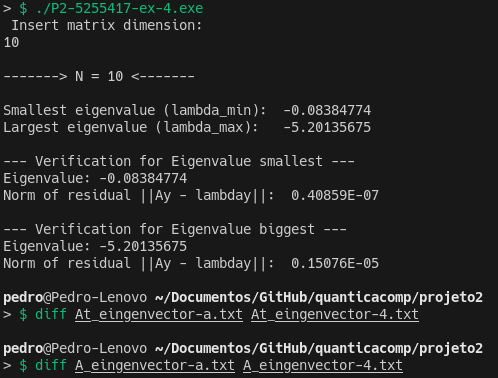
\includegraphics[width=0.8\textwidth]{../images/ex4.png}
        \end{figure}

        Nota-se que todas as verifica\c{c}\~oes resultaram em valores pequenos, comprovando que o c\'odigo permanece funcional , comprovando que o c\'odigo permanece funcional ---  mas utilizando significativamente menos mem\'oria. Al\'em disso, a pequena diferen\c{c}a em um elemento do vetor final pode ser atribu\'ida a problemas de aproxima\c{c}\~ao que ocorrem em ambos os c\'odigos --- n\~ao afetando a validade do resultado.

\end{document}